\documentclass[../main]{subfiles}
\begin{document}

\chapter{Private key encryption}

\section{Asymptotic approach}

\begin{definition}[PPT Algorithm]
    A probabilistic algorithm $A$ is said to be \textbf{Probabilistic Polynomial Time (PPT)} if there is a polynomial $p$ that defines an upper bound on the computation time
    of $A$ independently of the probabilistic choices made by the latter.
\end{definition}

\begin{definition}[Negligible function]
    A function $f: \mathbb{N} \rightarrow{} \mathbb{R}$ is said to be \textit{negligible} if and only if for every polynomial $p: \mathbb{N} \rightarrow{} \mathbb{N}$
    there exists $N \in{} \mathbb{N}$ such that for every $n > N$ it holds that $f(n) < \frac{1}{p(n)}$.
\end{definition}

\begin{lemma}[Closure of the set of negligible functions]
    \label{lemma:closure-ngl-functions}
    The set of all negligible functions, called $\mathcal{NGL}$, is closed for sum, product, and product by an arbitrary polynomial.
\end{lemma}

\paragraph{Proof}
Suppose $\varepsilon$ is a negligible function. Let $p: \mathbb{N} \rightarrow{} \mathbb{N}$ be any polynomial.\\
We want to prove that:
$$\varepsilon'(n) = \varepsilon(n)\cdot{}p(n)$$
is itself negligible.\\
We know that $\forall{} q: \mathbb{N} \rightarrow{} \mathbb{N}$ $\exists{} N \in{} \mathbb{N}\; s.t.\;\forall{} n > N$
$$\varepsilon(n) < \frac{1}{p(n)\cdot{}q(n)}$$
This is because $\varepsilon(n)$ is negligible and by definition is smaller than $\frac{1}{p(n)}$ and $\frac{1}{p(n)}$ hence also smaller than their product.
Let us prove that $\varepsilon'(n)$ is negligible, namely that $\forall{} q: \mathbb{N} \rightarrow{} \mathbb{N}$ $\exists{} N \in{} \mathbb{N}\; s.t.\;\forall{} n > N$
$$\varepsilon'(n) < \frac{1}{q(n)}$$
To conclude, we know that:
$$\varepsilon'(n) = \varepsilon(n) \cdot{} p(n) < \frac{1}{q(n)\cdot{}p(n)} \cdot{} p(n)$$
and therefore \ref{lemma:closure-ngl-functions} is proved.

\section{Proofs by reduction}

In the context of computational cryptography we have $|\mathcal{K}| \ll{} |\mathcal{M}|$ hence the adversary could construct ``easily'' two attacks:
\begin{itemize}
    \item (ciphertext-only) given a ciphertext $c$ the attacker could try to decrypt $c$ \textbf{with all possible keys} (it is a brute-force attack, of course, but perhaps feasible);
    \item (known-plaintext) given couples ($m_1$, $c_1$), ..., ($m_l$, $c_l$) the attacker could try to generate a key $k$ randomly and then check whether $Dec_k(c_i) = m_i$ for every $i$.
\end{itemize}
The probability of success of the attacker must be minimized, together with its computational power.
We would have to prove the following:
$$\forall{} A \in{} PPT \; \neg BRK(\Pi, A) \Leftrightarrow{} \nexists{} A \in{} PPT \; \neg BRK(\Pi, A)$$
in which $BRK(\Pi, A)$ means ``Algorithm/attacker A breaks scheme $\Pi$'', but that is currently impossible to prove.\\
The only thing we can prove right now is the following:
$$\forall{} B \in{} PPT \; \neg BRK(\Xi, B) \Rightarrow{} \forall{} A \in{} PPT \; \neg BRK(\Pi, A)$$
$$\Updownarrow$$
$$\exists{} A \in{} PPT \; BRK(\Pi, A) \Rightarrow{} \exists{} B \in{} PPT \; BRK(\Xi, B)$$
\begin{figure}[h]
    \centering
    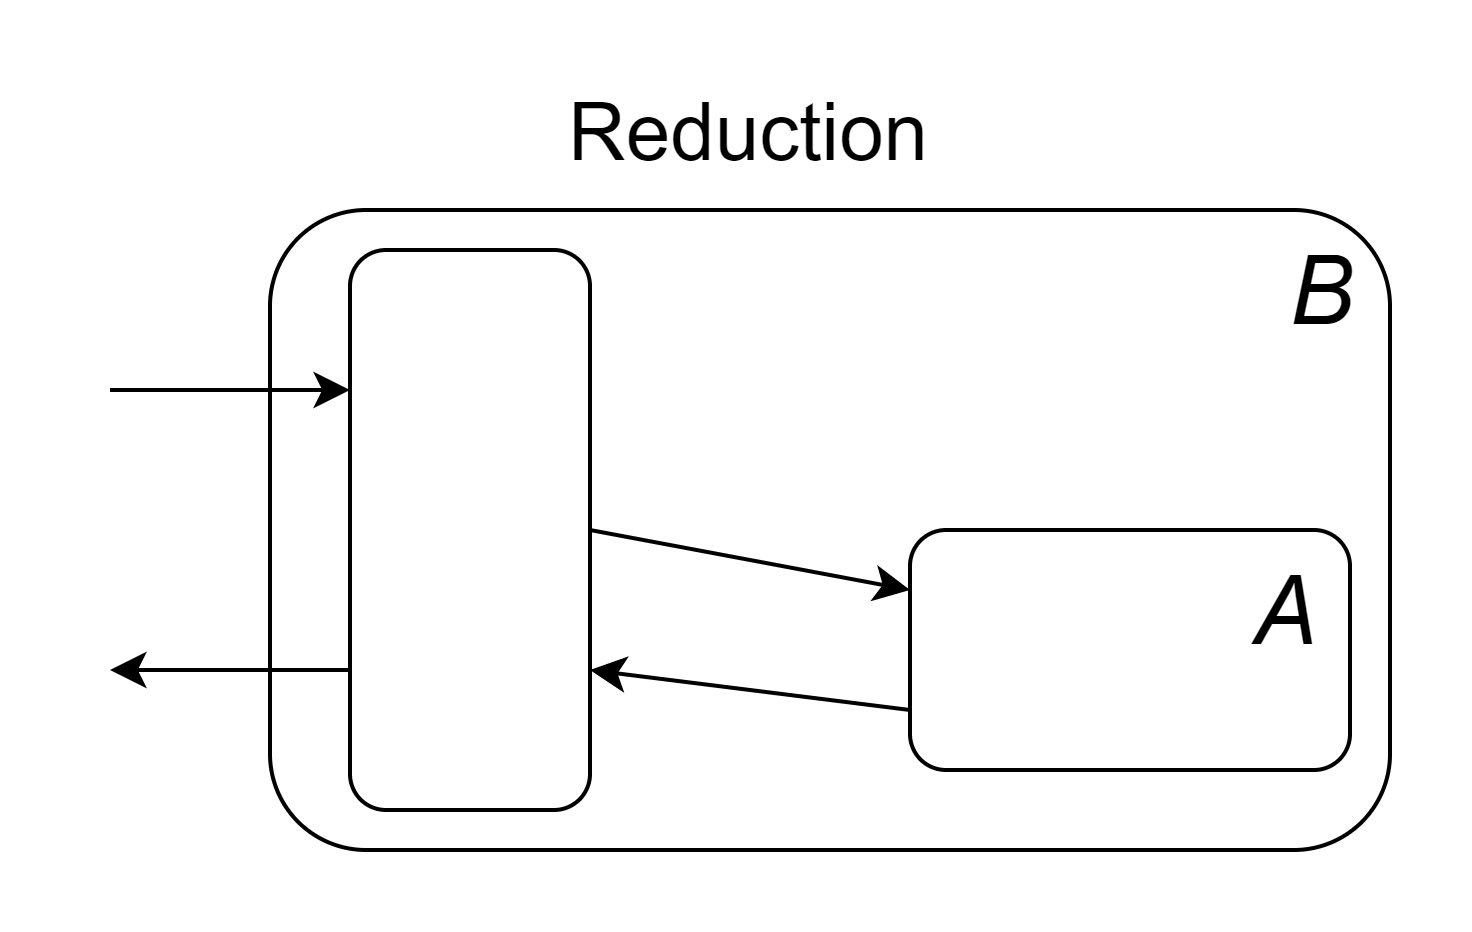
\includegraphics[width=0.5\textwidth]{images/reduction}
    \caption{Graphical representation of proofs by reduction.}
\end{figure}
\paragraph{Proof (by means of contradiction)}
Assuming that $\Xi$ is not solvable by efficient (PPT) algorithms, a part from those with negligible probability, we want therefore to prove that $\Pi$ is secure ($\forall{} B \in{} PPT \; \neg BRK(\Xi, B) \Rightarrow{} \forall{} A \in{} PPT \; \neg BRK(\Pi, A)$).\\
\begin{enumerate}
    \item Let's say that it exists $A \in PPT$, an efficient algorithm for solving $\Pi$ and that the probability of solving it is $\varepsilon(n)$ (which is a polynomial function).
    \item Now let's take $B \in{} PPT$, which is an efficient algorithm for solving $\Xi$, that uses $A$ as a subroutine internally without knowing how it works.
    It just knows how the inputs map to outputs. Given an instance $\xi$ of $\Xi$, $B$ simulates $\Pi$ for $A$; $A$ must not see any difference (inputs and outputs given to $A$ should respect the pre- and post-conditions of $\Pi$).
    If $A$ breaks $\Pi$ then $B$ should be able to solve $\Xi$ with instance $\xi$ with probability \textbf{at least} $\frac{1}{p(n)}$ (inverse polynomial).
    \item If $\varepsilon(n)$ is not negligible (which is not, because of assumptions made in step 1), then $B$ solves $\Xi$ with probability $\frac{\varepsilon(n)}{p(n)}$ which is not negligible (hence polynomial/efficient).
    Since $B$ is efficient, and we know that $A$ is efficient too, we showed that $B$ can solve $\Xi$ with non-negligible probability. Which is impossible because it violates the initial assumptions.
    \item To conclude, given the assumption on $\Xi$, no efficient algorithm $A$ can solve $\Pi$ with non-negligible probability $\varepsilon(n)$ and $\Pi$ is computationally secure. 
\end{enumerate}

\section{New definition of encryption scheme}
An encryption scheme in computational cryptography has the form $\Pi{} = (Gen, Enc, Dec)$ with $Gen, Enc, Dec \in{} PPT$ and:
\begin{itemize}
    \item $k \leftarrow{} Gen(1^n) \; s.t. \; |k| \ge{} n$. The parameter $n$ is regarded as the \textbf{security parameter};
    \item $Enc$ is probabilistic and therefore $Enc(m, k)$ can output different ciphertexts every time with the same couple $(m, k)$. Note that $k$ has no information on $n$ but it has been generated from it;
    \item $Dec$ is by the way purely deterministic, otherwise there would not be any way to get the original message $m$ from a given $c$;
    \item The scheme is correct: $Dec_k(Enc_k(m)) = m$;
    \item $Enc_k(m)$ can work with messages of length $l(n)$, where $n$ is the security parameter and $l$ is a function on it. For example, the OTP would have $l(n) = n$ (the identity function).
\end{itemize}
We need to update the experiment for understanding whether the scheme is secure:\\
$PrivK^{eav}_{A,\Pi}(n)$:\\
$(m_0,m_1) \; \leftarrow{} \; A(1^n)$\\
\textbf{if} $|m_0| \; \neq{} \; |m_1|$ \textbf{then}\\
\hspace*{20pt}\textbf{Result}: 0\\
$k \; \leftarrow{} \; Gen(1^n)$\\
$b \; \leftarrow{} \; \{0,1\}$\\
$c \; \leftarrow{} \; Enc(k,m_b)$\\
$b^* \; \leftarrow{} \; A(c)$\\
\textbf{Result}: $\neg(b \oplus{} b^*)$
\begin{definition}[Security of an encryption scheme]
    An encryption scheme $\Pi$ is said to be \textit{secure against passive attacks} (i.e., when the attacker does not know the $Enc$ and $Dec$ functions) or \textit{secure w.r.t.} $PrivK^{eav}$
    if and only if for each PPT adversary $A$ there exists a function $\varepsilon{} \in{} \mathcal{NGL}$ s.t.
    $$Pr(PrivK^{eav}_{A,\Pi}(n) = 1) = \frac{1}{2} + \varepsilon(n)$$
\end{definition}
As a note, $\frac{1}{2}$ corresponds to the probability we required also in the previous experiment. We are now adding only a negligible probability $\varepsilon(n)$.

\section{Pseudo randomness}
Since we cannot require anymore that $|\mathcal{M}| = |\mathcal{K}|$ and only that $|\mathcal{K}| < |\mathcal{M}|$ we must find a way to make the generated $k$ become of length $|m|$.
That is performed via a function $G$, which must be deterministic, efficiently computable, that expands $k$ without breaking the important properties of keys.\\
In particular, $G(k)$ must be \textbf{pseudo random}, i.e., an efficient adversary cannot distinguish it from a true random string.

\begin{definition}[Pseudo random generator]
    Let $l:\mathbb{N}\rightarrow{}\mathbb{N}$ be a polynomial, called \textit{expansion factor}, and let $G$ be a deterministic algorithm that $\forall{} s \in{} \{0,1\}^*$ (binary input strings) generates a string $G(s) \in{} \{0,1\}^{l(|s|)}$ (binary output strings of length $l(|s|)$).
    We say that $G$ is a \textit{pseudo random generator (GP)} if and only if:
    \begin{itemize}
        \item $\forall{}n \in{} \mathbb{N}$ it holds that $l(n) > n$ (i.e., $l$ cannot be the identity function like in the OTP).
        \item $G$ is polytime.
        \item For every PPT algorithm $D$ ($D$ stands for ``distinguisher") there exists $\varepsilon{} \in{} \mathcal{NGL}$ s.t. $|Pr(D(s) = 1) - Pr(D(G(r)) = 1)| \le{} \varepsilon(n)$ where $s$ and $r$ are (true) random strings; $s$ has length $l(n)$, $r$ has length $n$ and therefore $|G(r)|=l(n)$ (i.e., algorithm $D$ can understand that $G$ is not returning proper random strings only with negligible probability).
    \end{itemize}
\end{definition}

\begin{definition}[GP Induced Scheme]
    Given a GP $G$ with expansion factor $l$, the scheme $\Pi^G = (Gen,Enc,Dec)$ is defined as follows:
    \begin{itemize}
        \item The algorithm $Gen$ on input $1^n$ outputs each string of length $n$ with same probability, i.e., $\frac{1}{2^n}$.
        \item $Enc(m,k)=G(k)\oplus{}m$.
        \item $Dec(c,k)=G(k)\oplus{}c$.
        \item $\Pi^G$ produces messages with fixed length $l(n)$.
        \item Correctness is easy to prove: $Dec(Enc(m,k),k)=G(k)\oplus(G(k)\oplus m)=m$.
    \end{itemize}
\end{definition}

\begin{theorem}
    \label{theorem:pseudorandomgen-security}
    If $G$ is a pseudo random generator, then $\Pi^G$ is secure against passive attacks, namely secure w.r.t. $PrivK^{eav}$.
\end{theorem}

\paragraph{Proof (by reduction/contradiction)}
Let us assume that $\exists A$ attacker which breaks $\Pi^G$ according to $PrivK^{eav}$ and out of it let us build a distinguisher which wins over $G$.
Before defining the distinguisher $D$ let use write what we know about $A$:
$$Pr(PrivK^{eav}_{A,\Pi^G}(n) = 1) = \frac{1}{2} + \theta(n)$$
in which $\theta(n) \notin{} \mathcal{NGL}$.

\newpage
\begin{figure}[h]
    \centering
    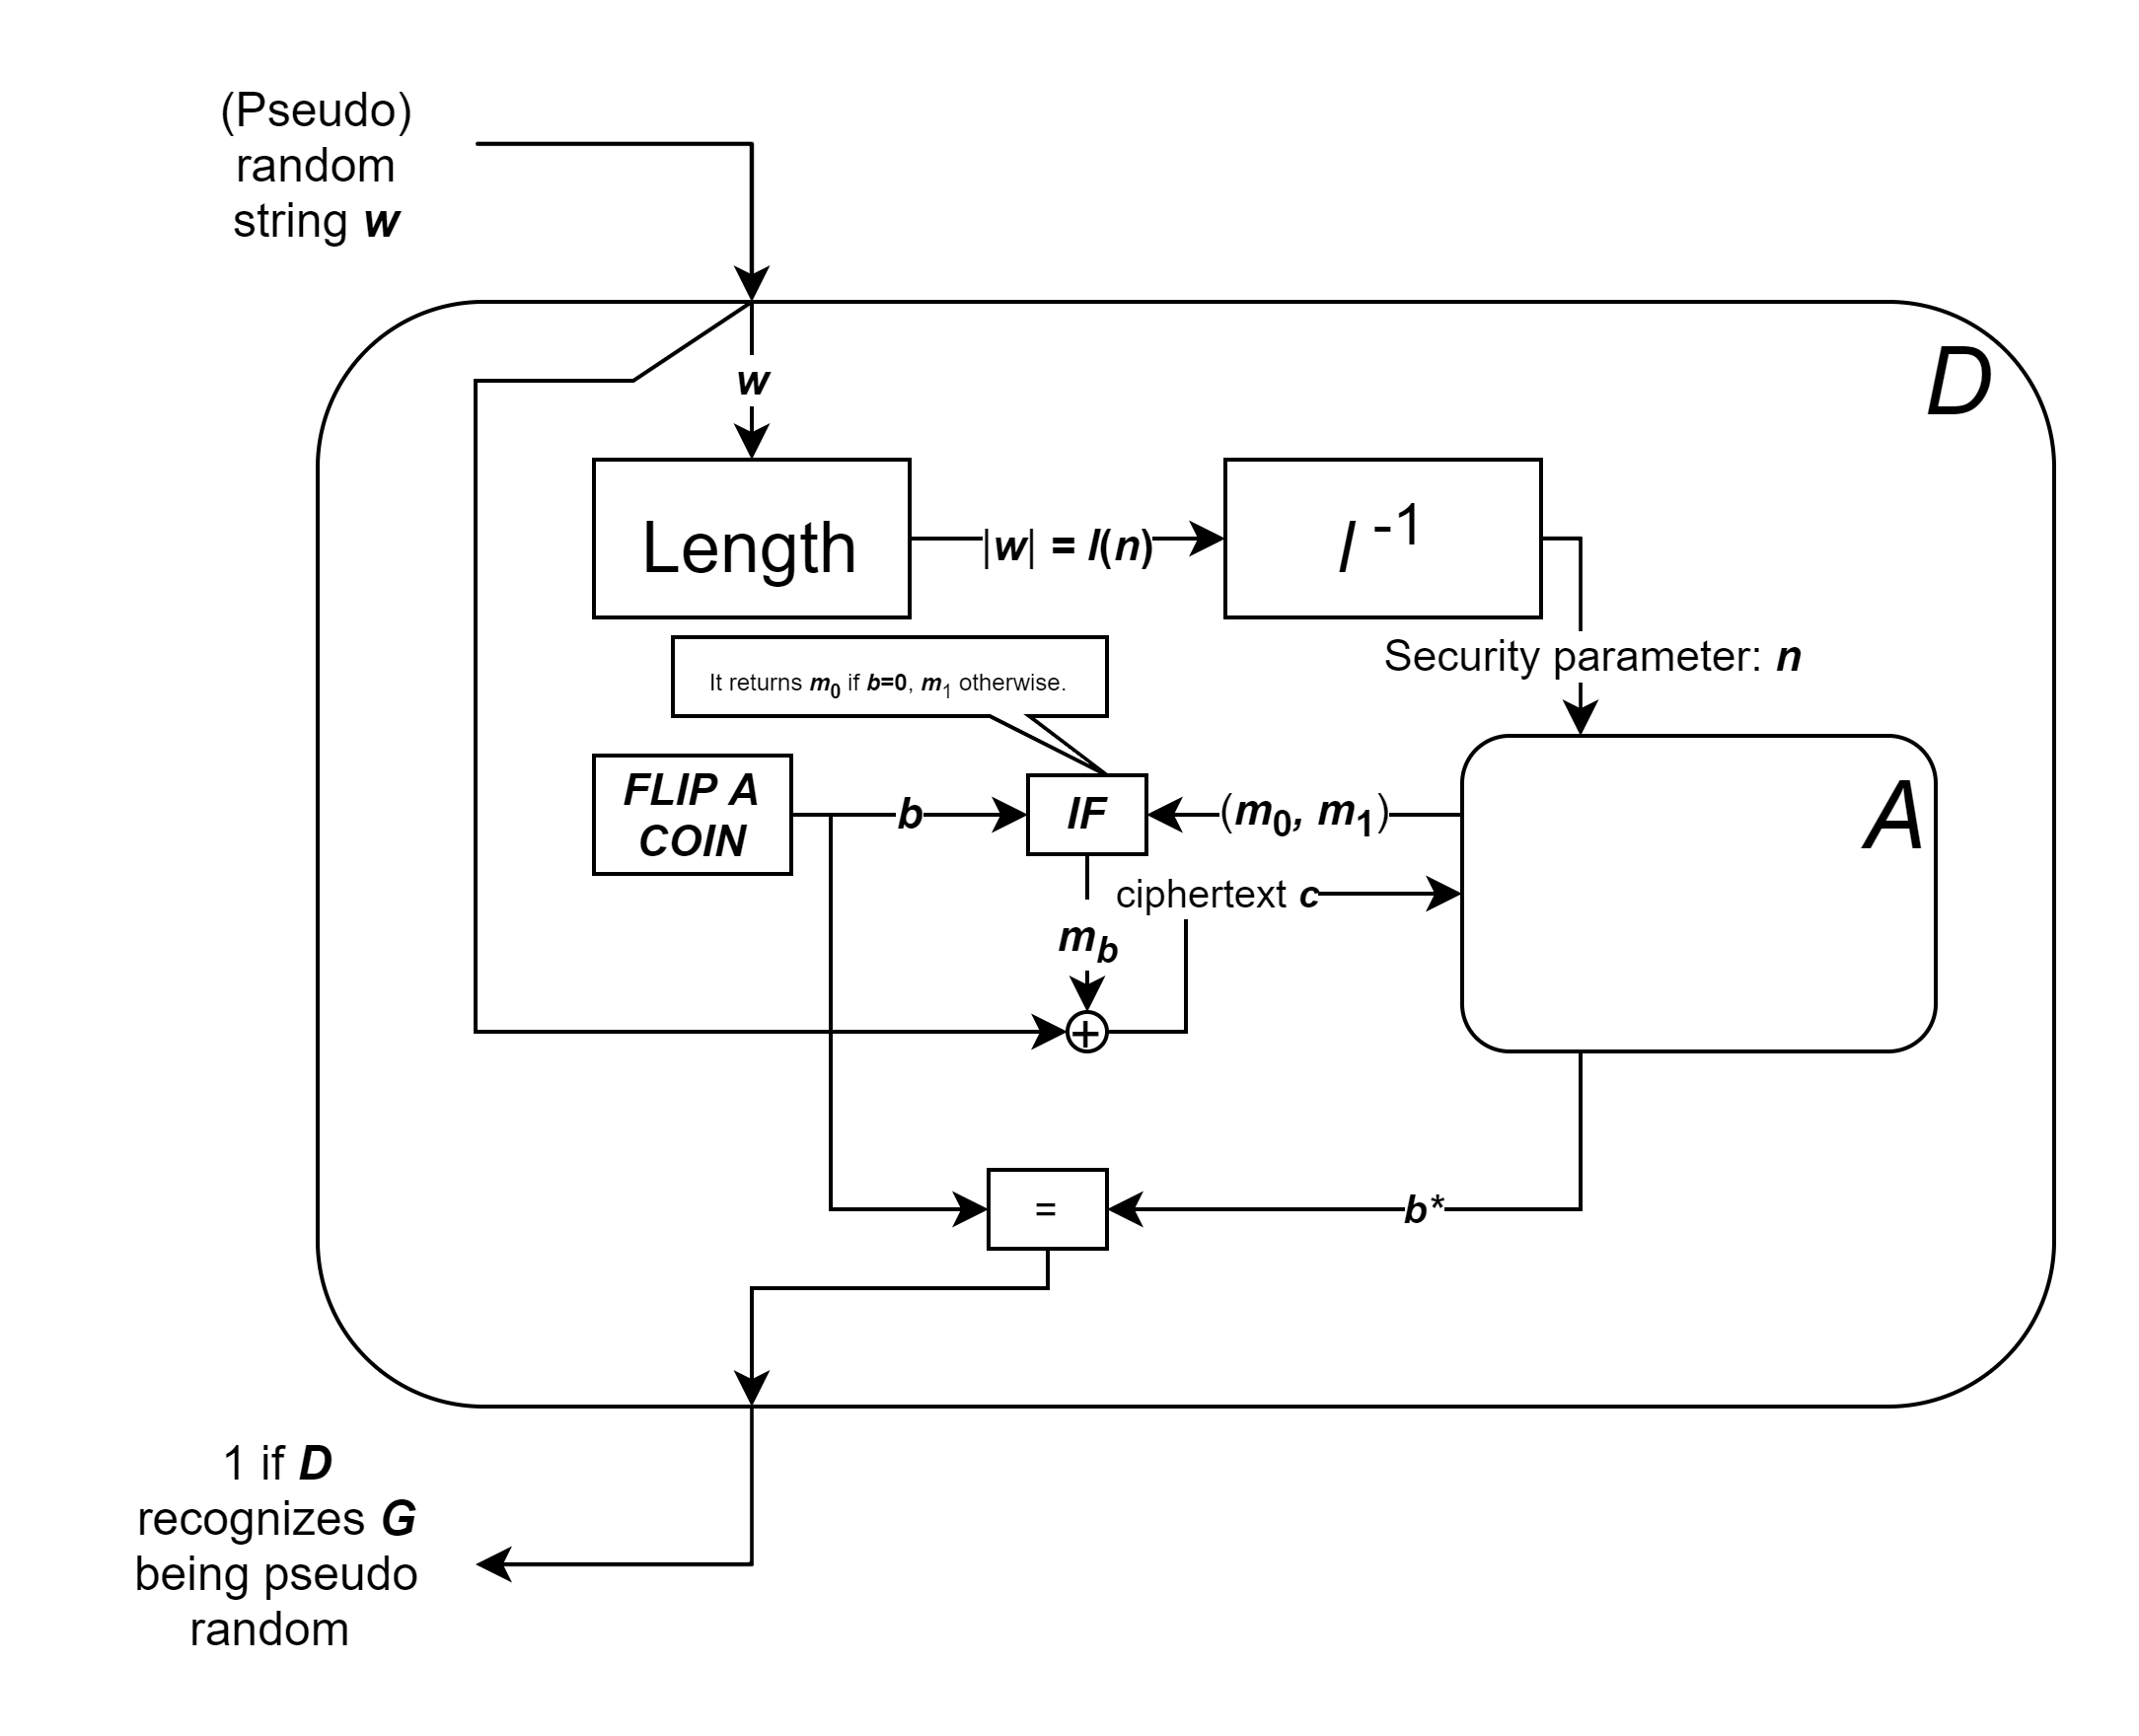
\includegraphics[width=0.5\textwidth]{images/security_of_pseudorandomgen}
    \caption{How the deterministic D can be generated out of an attacker A.}
\end{figure}
\noindent
Let us analyse the behaviour of the newly constructed $D$:
\begin{itemize}
    \item $Pr(D(G(r)) = 1) = Pr(PrivK^{eav}_{A,\Pi^G}(n) = 1)$ (note that $G(r)$ is exactly $w$ in the diagram explaining how $D$ is built);
    \item $Pr(D(s) = 1) = Pr(PrivK^{eav}_{A,OTP}(n) = 1)$ (note that $s$ is a purely random string, OTP is the One-Time Pad);
    \item $|Pr(D(G(r)) = 1) - Pr(D(s) = 1)| = |Pr(PrivK^{eav}_{A,\Pi^G}(n) = 1) - Pr(PrivK^{eav}_{A,OTP}(n) = 1)| = |(\frac{1}{2} + \theta(n)) - \frac{1}{2}| = |\theta(n)| = \theta(n)$
\end{itemize}
We are done: $\theta(n)$ is not negligible and this contradicts our hypothesis, hence we proved \ref{theorem:pseudorandomgen-security}.

\begin{definition}[Variable Output-Length Generators]
    A deterministic polytime algorithm $G$ is said to be \textbf{Variable Output-Length Generator} if from a seed $s \in{} \{0,1\}^n$ and a string in the form $1^l$ outputs a binary string $G(s,1^l)$ of length $l$ s.t.
    \begin{itemize}
        \item If $l < l'$, the string $G(s,1^l)$ is a prefix of $G(s,1^{l'})$.
        \item For any polynomial $p: \mathbb{N} \rightarrow{} \mathbb{N}$ (what we usually called $l$), the algorithm $G_p$ defined by setting $G_p(s)=G(s,1^{p(|s|)})$ is a pseudo random generator (of fixed length $p$).
        \item $Enc(m,k) = G(k, 1^{|m|}) \oplus m$.
        \item $Dec(c,k) = G(k, 1^{|c|}) \oplus c$.
    \end{itemize}
\end{definition}

\begin{lemma}
    For every pseudo random generator $G$ it is possible to construct from G a variable output-length pseudo random generator H.
\end{lemma}
\noindent
These so-called \textit{stream ciphers} are designed to satisfy axioms of Variable Output-Length Generators but \textbf{one cannot prove it} and \textbf{they are not encryption schemes}.

\section{Multiple encryptions}
\begin{lemma}
    The scheme $\Pi^G$ is not secure with respect to $PrivK^{mult}$, not even if $G$ is pseudo random.
\end{lemma}

\begin{theorem}
    If $Enc$ is deterministic, then the scheme $\Pi = (Gen, Enc, Dec)$ cannot be secure with respect to $PrivK^{mult}$.
\end{theorem}
\paragraph{Proof}
Let us describe an adversary $A$ which wins with high probability against any such scheme:
\begin{itemize}
    \item in the first phase, $A$ produces in output the two vectors (for example) $m_0 = (0^l, 0^l)$ and $m_0 = (0^l, 1^l)$;
    \item in the second phase, $A$ receives in input $c = (c_1, c_2)$, it compares $c_1$ and $c_2$ and produces in output $0$ if $c_1 = c_2$, $1$ otherwise;
    \item it is easy to see that $Pr(PrivK^{mult}_{A,\Pi}(n) = 1) = 1$ because $c_1 = c_2 \; \Leftrightarrow{} \; c = Enc(k,m_0)$ ($Enc$ is deterministic).
\end{itemize}

\noindent
Stream ciphers become useful again (right now they are useless, as we showed) when we give $Enc$ an \textbf{internal state} or we pass a so-called $Initialization \; Vector \; (IV)$.
\begin{figure}[h]
    \centering
    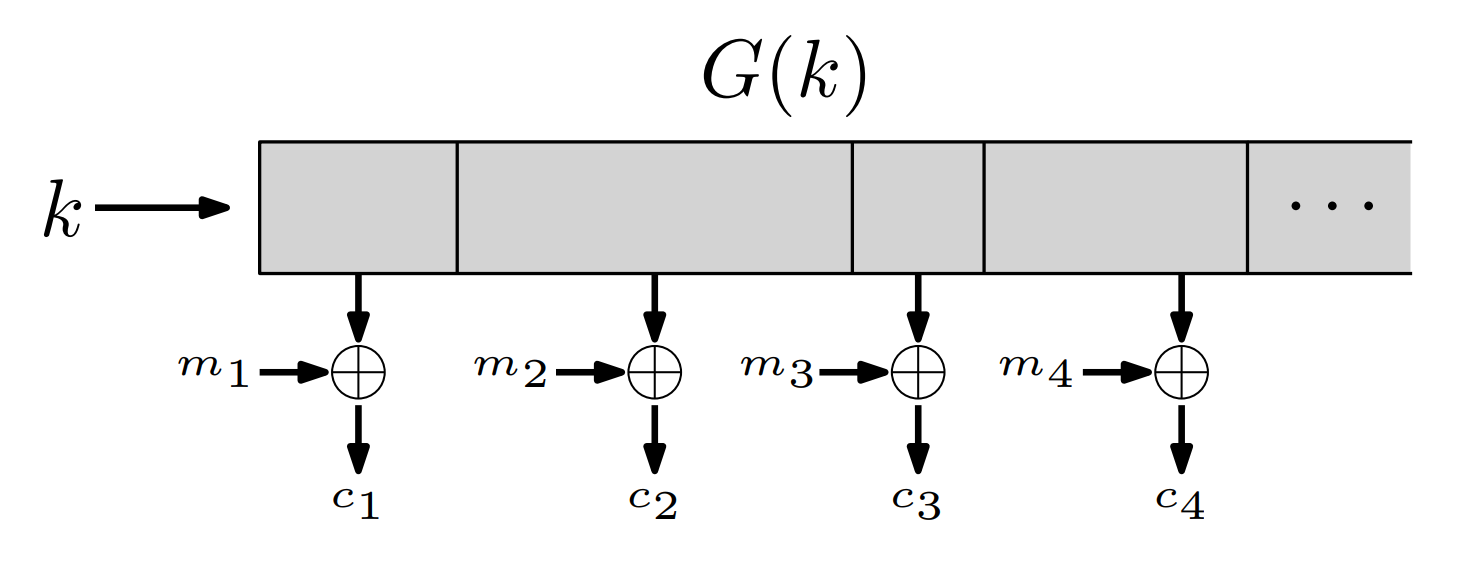
\includegraphics[width=0.5\textwidth]{images/synchronized_mode}
    \caption{Synchronized mode: Stream cipher with internal state (stateful).}
\end{figure}
\begin{figure}[h]
    \centering
    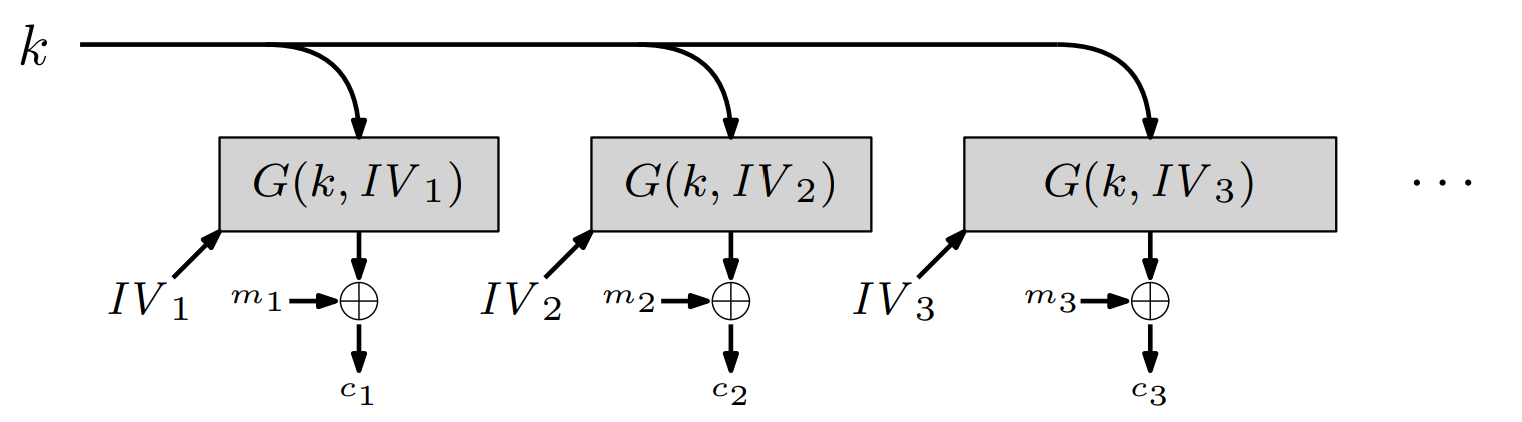
\includegraphics[width=0.5\textwidth]{images/unsynchronized_mode}
    \caption{Unsynchronized mode: Stream cipher without internal state (stateless).}
\end{figure}

\section{Security against Chosen Plaintext Attacks (CPA)}
The assumptions so far were that the attacks where only conducted in a safe manner, i.e., the attacker could not do much more than generate messages and check if they would match to a given ciphertext.
Right now the assumption we give is that the attacker has access to an \textbf{oracle} of $Enc_k$ for some given $k$.
The rest stays the same and the new experiment is called $PrivK^{CPA}$.

\begin{definition}[Security against CPA]
    An encryption scheme $\Pi$ is said to be secure against CPA attacks (or CPA-secure) if and only if for every adversary $A$ there exists $\varepsilon \in{} \mathcal{NGL}$ such that
    $$Pr(PrivK^{CPA}_{A,\Pi}(n) = 1) \leq{} \frac{1}{2} + \varepsilon(n)\footnote{This kind of definitions usually use strict equalities instead of inequalities: it is not important whether is the former or the latter, it's important the probability is approximately $\frac{1}{2}$.}$$
\end{definition}

\begin{lemma}
    Any scheme that is secure w.r.t. $PrivK^{CPA}$ is secure w.r.t. $PrivK^{eav}.$
\end{lemma}

\begin{lemma}
    Any scheme $\Pi{}=(Gen, Enc, Dec)$ that is secure w.r.t. $PrivK^{CPA}$ must be such that $Enc$ is probabilistic.
\end{lemma}

\begin{theorem}
    Every encryption scheme that is CPA-secure is secure even in case of multiple encodings.
\end{theorem}

\subsection{Constructing a CPA-secure cipher}

\subsubsection{Pseudo random functions}
Since $\Pi^G$ are pseudo random generators and are deterministic, there is no way they will ever be CPA-secure.
Therefore we will need to present the concept of \textbf{pseudo random functions}.
Some knowledge is needed before proceeding:
\begin{itemize}
    \item the concept of \textit{partial function} is required, i.e., functions defined in $\{0,1\}^*\times\{0,1\}^*\rightarrow\{0,1\}^*$;
    \item we are interested in partial functions because we want these functions to be \textbf{length preserving}, i.e., $F(k,x)$ is defined $\Leftrightarrow$ $|k| = |x|$, $|F(k,x)| = |x|$.
    \item given a length preserving function $F$ we call $F_k: \{0,1\}^{|k|} \rightarrow{} \{0,1\}^{|k|}$, where the first parameter is fixed and is $k$;
    \item a partial function is efficient if there exists a polytime algorithm computing it.
\end{itemize}
The space of these functions mapping $\{0,1\}^n \rightarrow{} \{0,1\}^n$ is huge but still finite:
\begin{itemize}
    \item every function has at most $2^n$ inputs and outputs string $n$-bit long, which creates a $(2^n \cdot{} n)$-sized table;
    \item like with binary strings, in which with $x$ bits we can express at most $2^x$ strings; in this space of functions, with $(2^n \cdot{} n)$ bits we can express a space of the following size: $2^{2^n \cdot{} n}$;
    \item every function can be chosen uniformly randomly: $\frac{1}{2^{2^n \cdot{} n}}$.
\end{itemize}

\begin{definition}
    Given a binary partial function $F$, which is length preserving and efficiently computable, 
    we say that $F$ is a pseudo random function (FP) if and only if for every PPT distinguisher $D$ 
    there exists a negligible function $\varepsilon$ such that
    $$|Pr(D^{F_k(\cdot)}(1^n)=1)-Pr(D^{f(\cdot)}(1^n)=1)|\le{}\varepsilon(n)$$
    where $k$ is chosen among all strings of length $n$ and $f(\cdot)$ (truly random function) is chosen among all functions in $\{0,1\}^n \rightarrow{} \{0,1\}^n$.
\end{definition}

\noindent
By the way, as with pseudo random functions are not proved to exist like with pseudo random generators.
There are constructions that are meant to satisfy axioms of pseudo random functions, but again, they are not proved; these are the so-called \textbf{block ciphers} (e.g., DES or AES).

\begin{definition}[FP Induced Scheme]
    Given a FP $F$, the scheme $\Pi^F = (Gen,Enc,Dec)$ is defined as follows:
    \begin{itemize}
        \item The algorithm $Gen$ on input $1^n$ outputs each string of length $n$ with same probability, i.e., $\frac{1}{2^n}$.
        \item $Enc(m,k)$ is defined as the (binary encoding of the) pair $\langle r, F_k(r)\oplus m \rangle$ where $r$ is a truly random bit string with length $k$.
        \item $Dec(c,k)$ returns $F_k(r)\oplus s$ anytime $c$ is the (binary encoding of the) pair $\langle r, s \rangle$.
        \item Correctness is easy to prove: $Dec(Enc(m,k),k)=F_k(r)\oplus(F_k(r)\oplus m)=m$ (given a truly random generated $r$).
    \end{itemize}
    $F_k$ is length preserving and can only be applied to messages of length equal to the value returned by $F_k$.
    There are ways to generalize this scheme, shown below.
\end{definition}
Therefore $Enc(m,k)$ depends on the generated value of $r$, which means that different invocations of $Enc$ return different results.

\begin{theorem}
    If $F$ is FP, then $\Pi^F$ is secure against CPA attacks (i.e., it is CPA-secure).
\end{theorem}

\begin{definition}[FP Induced Scheme handling variable-length messages]
    Given a CPA-secure cipher $\Pi$ for messages of length $n$, a generalization for messages of length $l(n)$ (where $l$ is a polynomial on $n$) is obtained but slightly modifying $Enc$ (and of course $Dec$ follows):
    $$Enc^*(k, m_0 || ... || m_{l(n)}) = Enc(k,m_0) || ... || Enc(k,m_{l(n)})$$
\end{definition}

\begin{theorem}
    If $\Pi$ is CPA-secure, then $\Pi^*$ is also CPA-secure.
\end{theorem}

\subsubsection{Pseudo random permutations}
A permutation of a set $X$ is a just a bijective (i.e., invertible) function $F: X \rightarrow{} X$.
The number of possible permutations is big ($(2^n)!$), but smaller than the space of functions (which was $2^{2^n \cdot{} n}$).
Both $F$ and $F^{-1}$ are required to be efficiently computable and since sometimes the adversaries have access to both of them, it makes sense to require the following:
$$|Pr(D^{F_k(\cdot),F^{-1}_k(\cdot)}(1^n)=1)-Pr(D^{f(\cdot),f{-1}(\cdot)}(1^n)=1)| \le{} \varepsilon(n)$$
which is the notion of \textbf{strongly pseudo random permutation}.\\
\noindent
The previously nominated \textbf{block ciphers} are also thought to be strongly pseudo random permutations.

\subsubsection{Modes of operation}
The construction $\Pi$ is just one of many ways in which a block cipher can be used to construct an encryption scheme.
In literature, this is referred as \textbf{mode of operation}: each of these assumes the message $m$ to be split in $m_0$, ..., $m_l$, each of them of length $|k|$ (assuming also that $|m|$ is a multiple of $|k|$).
Some modes of operations are the following:
\begin{itemize}
    \item \textbf{Electronic Code Book (ECB)}, which is secure for passive attacks but not CPA-secure;
    \item \textbf{Cipher Block Chaining (CBC)}, which is unfortunately not parallelizable (since to encode the $i$-th partial message $m_i$ is required $c_{i-1}$);
    \item \textbf{Output FeedBack (OFB)}, which is partially parallelizable ($F_k$ computation is parallelizable, the encoding is not);
    \item \textbf{Counter (CTR)}, which is parallelizable (and C is sent in the channel with the ciphertext).
\end{itemize}
\end{document}